\documentclass{article}

\usepackage{geometry}
\geometry{
	a4paper,
	total={170mm,257mm},
	left=20mm,
	top=20mm,
}
\usepackage{authblk}
\usepackage[utf8]{inputenc}
\usepackage{amssymb,amsmath}
\usepackage[english]{babel}
\usepackage[T1]{fontenc}
\usepackage{enumerate}
\usepackage{dsfont}\let\mathbb\mathds
\usepackage[all]{xy}
\usepackage{fancyhdr}
\usepackage{hyperref}
\usepackage{url}
\usepackage{float} %float
\floatstyle{plaintop}
\restylefloat{table}
\usepackage{caption}
%\usepackage[aboveskip=1pt,labelfont=bf,labelsep=period,singlelinecheck=off]{caption}
\usepackage{multirow}
\usepackage{tabularx}
\usepackage{listings}
\usepackage{color}
\usepackage{booktabs}
\usepackage{multirow}

\usepackage{scalerel}
\usepackage{systeme}
\usepackage{listings}
\usepackage{color}
\usepackage{upgreek}
\usepackage{graphicx}
\usepackage{ragged2e}
\usepackage{makecell}

\newcommand{\bbN}{\mathbb{N}}
\newcommand{\bbZ}{\mathbb{Z}}
\newcommand{\bbQ}{\mathbb{Q}}
\newcommand{\bbR}{\mathbb{R}}
\newcommand{\bbC}{\mathbb{C}}
\newcommand{\intf}{\int_{-\infty}^{+\infty}}
\allowdisplaybreaks

%\renewcommand{\thesection}{S\arabic{section}}
%\renewcommand{\thetable}{S\arabic{table}}
%\renewcommand{\thefigure}{S\arabic{figure}}


\newcommand*{\toccontents}{\@starttoc{toc}}
\bibliographystyle{vancouver}



\newcommand\numberthis{\addtocounter{equation}{1}\tag{\theequation}}

\renewcommand{\headrulewidth}{0pt}
\renewcommand{\footrulewidth}{0.4pt}
\fancyhead[RO,LE]{}
\fancyhead[LO,RE]{Anthony Hauser  \& al.}
\fancyfoot[RO,LE]{\thepage}
\fancyfoot[LO,RE]{\textsc{Supplementary Material}}
\fancyfoot[C]{\today}
\pagestyle{fancy}
\setlength{\parindent}{0cm}
\newcommand{\HRule}{\rule{\linewidth}{0.5mm}}


\title{\textsc{\LARGE Supplementary material}\\[0.5cm]
\HRule \\[0.1cm]{\Large \bfseries The Impact of Scaling up Dolutegravir on Antiretroviral Resistance in South Africa  \\[-0.1cm] }\HRule}


\author[1]{Anthony Hauser}
\author[2]{Katharina Kusejko}
\author[3]{Leigh Johnson}
\author[2,4]{Huldrych Günthard}
\author[1]{Julien Riou}
\author[1,5]{Gilles Wandeler}
\author[1,3,*]{Matthias Egger}
\author[2,4,*]{Roger Kouyos}
\affil[1]{{\small Institute of Social and Preventive Medicine, University of Bern, Switzerland}}
\affil[2]{{\small Division of Infectious Diseases and Hospital Epidemiology, University Hospital Zurich, University of Zurich, Zurich, Switzerland}}
\affil[3]{{\small Centre for Infectious Disease Epidemiology and Research, University of Cape Town, South Africa}}
\affil[4]{{\small Institute of Medical Virology, University of Zurich, Zurich, Switzerland}}
\affil[5]{{\small Department of Infectious Diseases, Bern University Hospital, University of Bern, Bern, Switzerland}}
\affil[*] {{\small Corresponding  authors (\texttt{matthias.egger@ispm.unibe.ch}, \texttt{roger.kouyos@uzh.ch})}}


\begin{document}

\maketitle
	
	\vspace{-3em}
	
\tableofcontents

\clearpage

\section{Adapted MARISA model}\label{marisa}
\subsection{MARISA model}
MARISA is a mechanistic, compartmental model developed to capture the dynamics of HIV NNRTI resistance among adults in South Africa over the years 2005-2016. It models the continuum of care - including NNRTI-based first-line and PI-based second-line regimens -, the disease progression, acquisition and transmission of NNRTI-resistance, and its impact on the efficacy of NNRTI-based regimen. The model was calibrated using different sources of data: 1) cohort data about more than 54,000 people living with HIV from IeDEA collaboration \cite{Egger2012}, 2) data from literature, and 3) general HIV estimates at the country scale produced by the Thembisa model. The Thembisa model is a compartmental model providing UNAIDS with estimates on the South African HIV epidemic \cite{Johnson2017b}.

We adapted this model to investigate the impact of the introduction of DTG-based regimens in South Africa from 2020. The changes include 1) incorporating DTG-based regimen into the continuum of care, 2) distinguishing between DTG-eligible and -ineligible individuals, and 3) adding a NRTI-resistance dimension.

\subsection{Adapted MARISA model}
The adapted MARISA model is split in 5 dimensions: 1) care stages (15 levels), 2) disease progression, characterised by the CD4 counts (4 levels), 3) gender (2 levels), 4) NNRTI resistance (2 levels) and 5) NRTI resistance (2 levels).

The first dimension of the model accounts for the whole continuum of care (see Fig \ref{figure1}). The first three compartments model respectively HIV-infection of susceptible individuals and diagnosis (with a distinction between DTG-eligible and -ineligible women). We then considered the three different regimens - NNRTI-based, PI-based and DTG-based -, again with a distinction by DTG-eligibility for individuals on a NNRTI-based regimen. For each of the three regimens, three compartments are used to model treatment initiation ("Treat init.") with subsequent virological suppression ("Supp") or failure ("Fail").
"Treat init." compartments represent individuals who initiated treatment less than 3 months ago. Before 2020, all individuals receive a NNRTI-base first-line regimen and switch to the second-line PI-based regimen in case of prolonged failure. From 2020, the DTG-based regimen is used as a first-line regimen for all DTG-eligible individuals. From this time, DTG-eligible individuals who are currently on NNRTI-based regimen can transition to DTG-based regimen. PI-based regimen is still used as a second-line regimen, either for DTG-ineligible patients failing NNRTI-based ART, or for patients failing DTG-based ART.
%Patients failing NNRTI-based ART who are eligible for DTG switch to DTG-based ART.

\begin{figure}[h]
   \includegraphics[width=16cm]{../../dtg_latex_roger/figures/dtg_graph_cropped.pdf}
   \caption{Adapted MARISA model. Only the first (continuum of care) and the third (gender) dimensions are represented.}\label{figure1}
\end{figure}

The second dimension splits individuals in 4 classes according to CD4 counts: 1) $CD4>500 \text{ cells}/\mu L$, 2) $350<CD4<500 \text{ cells}/\mu L$, 3) $200<CD4<350  \text{ cells}/\mu L$ and 4) $CD4<200  \text{ cells}/\mu L$.  The third dimension makes the distinction between male and female. The fourth and fifth dimensions respectively model NNRTI- and NRTI-resistance. They each have two layers that distinguish between NNRTI-/NRTI-susceptible and -resistant individuals. We used the following indices to indicate a layer of a dimension: $j$ for the second dimension ($j=1,2,3,4$), $k$ for the third dimension ($k=1,2$), $l$ for the fourth dimension ($l=1,2$) and $m$ for the fifth dimension ($m=1,2$).
\newpage
\section{Parameters and rates of the adapted MARISA model}
\subsection{Rates related to continuum of care and disease progression}
Rates related to disease progression $\nu_{CD4}$ and $\tilde{\nu}_{CD4}$ as well as rates related to continuum of care $\gamma$, which respectively model transition from one to another CD4 class and transition from one to another care stage, were estimated using observational cohort data from IeDEA-SA collaboration. Survival analyses were performed using information of more than 54'000 patients from South Africa. Mean estimates and 95\% confidence intervals (95\%CI) are reported in Table \ref{tab1} and \ref{tab2}.

\begin{table}[H]
\centerline{
	\begin{tabular}{
	>{\RaggedRight\arraybackslash}p{0.1\textwidth}
	>{\RaggedRight\arraybackslash}p{0.5\textwidth}
	>{\RaggedRight\arraybackslash}p{0.0\textwidth}
	>{\RaggedRight\arraybackslash}p{0.12\textwidth}
	>{\RaggedRight\arraybackslash}p{0.12\textwidth}
	>{\RaggedRight\arraybackslash}p{0.12\textwidth}}
		\hline
		Parameter & Description & & \multicolumn{3}{c}{Values [95\% CI]}\\ 
		\hline\\[-0.4cm]
		\multicolumn{2}{l}{\textit{Parameters related to disease progression}}\\
		& & & \multicolumn{3}{c}{CD4 class}\\
		& & & $1\rightarrow 2$ & $2\rightarrow 3$ & $3\rightarrow 4$\\
		\cmidrule(lll){4-6}\\[-0.2cm]
		$1/\nu_{CD4}^{I}$ & Average time to progress from one to another CD4 class, at $I$ (taken from \cite{Mangal2017}) & & 60 & 36 & 42\\
		$1/\nu_{CD4}^{D}$ & Average time to progress from one to another CD4 class, at $D$ (taken from \cite{Mangal2017}) & & 60 & 36 & 42\\
		
$1/\nu_{CD4}^{T_1}$ & Average time to progress from one to another CD4 class, at $T_1$ &   & 47 [42,54] & 30 [28,34] & 60 [55,66] \\ 
  $1/\nu_{CD4}^{F_1}$ & Average time to progress from one to another CD4 class, at $F_1$ &   & 18 [16,20] & 15 [14,16] & 22 [21,24] \\ 
  $1/\nu_{CD4}^{T_2}$ & Average time to progress from one to another CD4 class, at $T_2$ &   & 32 [14,72] & 22 [12,43] & 33 [17,64] \\ 
  $1/\nu_{CD4}^{F_2}$ & Average time to progress from one to another CD4 class, at $F_2$ &   & 14 [8,26] & 15 [8,27] & 16 [10,25] \\  [0.5cm]
  
		& & & $1\leftarrow 2$ & $2\leftarrow 3$ & $3\leftarrow 4$\\
		\cmidrule(lll){4-6}\\[-0.2cm]
		
$1/\tilde{\nu}_{CD4}^{T_1}$ & Average time to progress from one to another CD4 class, at $T_1$ &   & 16 [15,17] & 16 [15,17] & 18 [17,19] \\ 
  $1/\tilde{\nu}_{CD4}^{S_1}$ & Average time to progress from one to another CD4 class, at $S_1$ &   & 17 [16,17] & 14 [14,14] & 9 [9,10] \\ 
  $1/\tilde{\nu}_{CD4}^{T_2}$ & Average time to progress from one to another CD4 class, at $T_2$ &   & 16 [9,27] & 19 [11,31] & 41 [23,73] \\ 
  $1/\tilde{\nu}_{CD4}^{S_2}$ & Average time to progress from one to another CD4 class, at $S_2$ &   & 17 [13,21] & 14 [11,17] & 7 [6,10] \\ 
  
		\hline\\[-0.4cm]
	\end{tabular}
}
\caption{Rates related to disease progression. Rates are in $\text{month}^{-1}$.}
\label{tab1}
\end{table}

\setlength{\tabcolsep}{10pt}
\begin{table}[H]
\centerline{
	\begin{tabular}{l
	p{0.25\textwidth}
	p{0.12\textwidth}
	p{0.14\textwidth}
	p{0.12\textwidth}
	p{0.12\textwidth}
}
		\hline
		Parameter & Description & \multicolumn{3}{c}{Values [95\% CI]}\\ 
		\hline\\[-0.4cm]
		\multicolumn{2}{l}{\textit{Parameters related to care stages}}\\
		&  &\multicolumn{4}{c}{CD4 class}\\
		&  & $1$ & $2$ & $3$ & $4$\\
		\cmidrule(llll){3-6}\\[-0.2cm]
		$1/\gamma_{T_1\rightarrow S_1}$ & Time from $T_1$ to $S_1$ & \makecell{3.4\\[0cm]  [3.3,3.6]} & \makecell{3.5\\[0cm]  [3.3,3.7]} & \makecell{3.6\\[0cm]  [3.4,3.7]} & \makecell{3.9\\[0cm]  [3.8,4.1]} \\ 
  $1/\gamma_{T_1\rightarrow F_1}$ & Time from $T_1$ to $F_1$ & \makecell{23.4\\[0cm]  [20.1,27.3]} & \makecell{22.8\\[0cm]  [19.6,26.4]} & \makecell{18.9\\[0cm]  [17.5,20.4]} & \makecell{12.9\\[0cm]  [12.3,13.5]} \\ 
  $1/\gamma_{S_1\rightarrow F_1}$ & Time from $S_1$ to $F_1$ & \makecell{176.3\\[0cm]  [157,197.9]} & \makecell{133.8\\[0cm]  [118.6,150.8]} & \makecell{62.1\\[0cm]  [57,67.6]} & \makecell{22.1\\[0cm]  [20.2,23.9]} \\ 
  $1/\gamma_{F_1\rightarrow S_1}$ & Time from $F_1$ to $S_1$ & \makecell{6.4\\[0cm]  [5.5,7.4]} & \makecell{12.9\\[0cm]  [11,14.9]} & \makecell{14.3\\[0cm]  [12.9,15.9]} & \makecell{18.2\\[0cm]  [16.3,20.2]} \\ 
  $1/\gamma_{F_1\rightarrow T_2}$ & Time from $F_1$ to $T_2$ & \makecell{467.5\\[0cm]  [243,898.9]} & \makecell{376\\[0cm]  [240.4,589.9]} & \makecell{258.9\\[0cm]  [200.7,334.6]} & \makecell{166.4\\[0cm]  [140,199]} \\
  $1/\gamma_{T_2\rightarrow S_2}$ & Time from $T_2$ to $S_2$ & \makecell{3.8\\[0cm]  [2.7,5.2]} & \makecell{3.8\\[0cm]  [2.6,5.5]} & \makecell{4\\[0cm]  [3,5.3]} & \makecell{5\\[0cm]  [4,6.4]} \\ 
  $1/\gamma_{T_2\rightarrow F_2}$ & Time from $T_2$ to $F_2$ & \makecell{14.3\\[0cm]  [7.8,26.8]} & \makecell{14\\[0cm]  [7.3,27]} & \makecell{11.8\\[0cm]  [7.8,18]} & \makecell{7.6\\[0cm]  [5.9,9.9]} \\ 
  $1/\gamma_{S_2\rightarrow F_2}$ & Time from $S_2$ to $F_2$ & \makecell{61.4\\[0cm]  [30.8,122.8]} & \makecell{40.9\\[0cm]  [21.4,78.9]} & \makecell{40\\[0cm]  [21.4,74.3]} & \makecell{19.1\\[0cm]  [9,40]} \\ 
  $1/\gamma_{F_2\rightarrow S_2}$ & Time from $F_2$ to $S_2$ & \makecell{2.3\\[0cm]  [1.1,4.1]} & \makecell{12.9\\[0cm]  [3.2,51.3]} & \makecell{5.5\\[0cm]  [2.8,11.3]} & \makecell{11.7\\[0cm]  [4.8,28]} \\ 
		\hline
	\end{tabular}
}
\caption{Rates related to transition between care stages. Rates are in $\text{month}^{-1}$.}
\label{tab2}
\end{table}

\subsection{Diagnosis, treatment initiation and switching rates}
Diagnosis rates depend on gender and CD4 classes and treatment initiation rates depend on CD4 classes. They have been described in details in \cite{Hauser2019}, S1 File, Section 1.3. In the adapted MARISA model, we assumed that diagnosis rates are constant from 2016, while the treatment initiation rate has been adapted in order to model the impact of the Treat-All policy. We increased treatment initiation rates for the first three first CD4 count classes from 2017 to 2022 in order to have identical rates irrespective of CD4 counts from 2022 (see Fig \ref{fig_treatrate}). To ensure a proportion $p_1$ of DTG-eligible women, two diagnosis rates are used $\gamma_{I\rightarrow D}^{k,elig}:=p_1\cdot\gamma_{I\rightarrow D}^{k}$, $\gamma_{I\rightarrow D}^{k,inel}:=(1-p_1)\cdot\gamma_{I\rightarrow D}^{k}$, in order to distribute women into the two DTG-eligibility classes.

\begin{figure}[h]
   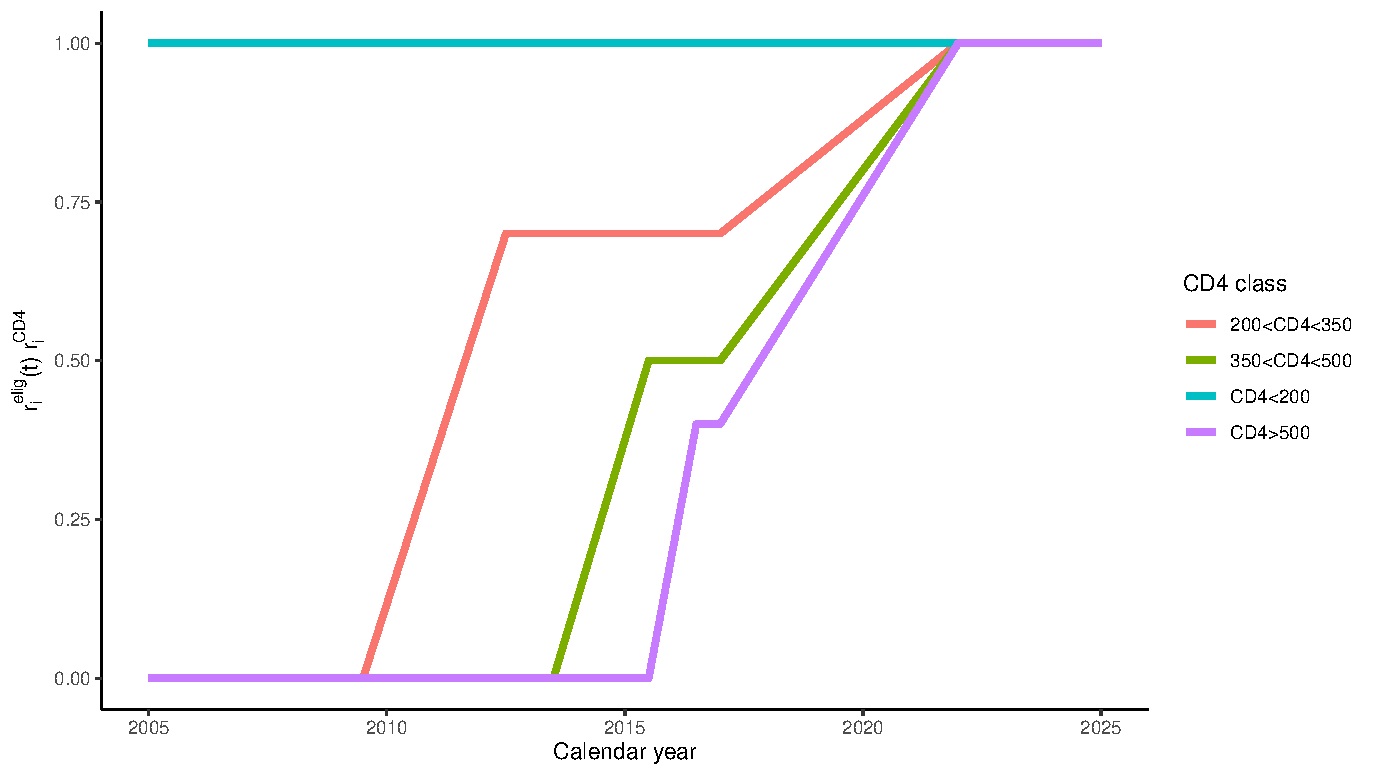
\includegraphics[width=16cm]{../figures/dtg_treatrate.pdf}
\caption{$r^{elig}_i(t) \cdot r^{CD4}_i$ represents the level of treatment eligibility $r^{elig}_i(t)$ multiplied by $r^{CD4}_i$, representing the lower treatment initiation rate of CD4 class $i$ relative to the CD4 class $i=4$. These two components are parts of the overall treatment initiation rate $\gamma_{D\rightarrow T_1}^i (t)=\gamma^{CD4<200}_{2005} \cdot r^{elig}_i(t) \cdot r^{CD4}_i \cdot r^{time}(t)$.}\label{fig_treatrate}
\end{figure}

We rescaled the switching rates from unsuppressed NNRTI-based regimen to PI-based regimen $\gamma_{F_1\rightarrow T_2}^{k,elig/inel}$ in order to reflect PI-coverage in South Africa ($\sim 4\%$ in 2016 according to \cite{Moorhouse2019}). The new rates $\gamma_{F_1\rightarrow T_2}^{k,elig/inel}$ can be found in Table \ref{tab2}.


\subsection{Resistance rates}
Two rates model the flow between the two NNRTI-resistance layers: the reversion rate $\sigma_{rev}$ and the rate of acquiring NNRTI-resistance $\sigma_{res}^{NNRTI}$. Reversion to wild-type occurs when no more drug pressure is exerted, i.e. in the "Infected" and "Diagnosed" compartments. An individual can acquire NNRTI-resistance when failing first-line regimen. Both parameters $\sigma_{rev}$ and $\sigma_{res}^{NNRTI}$ were collected from literature and can be found in Table \ref{tab:literature}.

\begin{table}[H]
\caption{Parameters collected from literature. As mortality estimates in the fourth CD4 class vary according to the proportion of people with $CD4<50\text{ cells}/\mu L$, lower and upper bounds are given (see \cite{Hauser2019} S1 File Section 1.2 for more details). The mortality risk $\mu^{j}_{X}$ in CD4 class $j$ ($i=1,\ldots,4$) and care stage $X$ ($X=I,D,T_1,\ldots$) is given by: $\mu^{j}_{X}=\mu_0\cdot\tilde{\mu}^{j}_{X}$.}
\label{tab:literature}
\centerline{
\begin{tabular}{llllll}
		\hline\\[-8pt]
		Parameter & Description & Values & Ref \\[1pt]
		\hline\\[1pt]
		\multicolumn{2}{l}{\textit{Resistance parameters}}\\
		$1/\sigma^{NNRTI}_{res}$ & Time to acquire NNRTI-resistance (in month) & 5 & \multicolumn{2}{l}{\cite{res,Sigaloff2012,Wallis2010,Manasa2013,VanZyl2011}}\\
		$1/\sigma^{NRTI}_{res}$ & Time to acquire NRTI-resistance (in month) & 40 & \multicolumn{2}{l}{\cite{Hauser_github}}\\
		$1/\sigma_{rev}$ & Time to revert back to wild-type (in month) & 125 & \cite{rev}\\

		$\alpha_1$ & Impact of NNRTI-resistance on NNRTI-based ART & 1.97 & \cite{Wittkop2011,Kuritzkes2008}\\
		$\alpha_2$ & Impact of NNRTI-resistance on NNRTI-based ART & 3.24 & \cite{Wittkop2011,Kuritzkes2008}\\
		$\alpha_3$ & Impact of NRTI-resistance on DTG-based ART & 1 & \cite{Hakim2018,Giacomelli2019,F1000Research}\\
		$\alpha_4$ & Scaling factor for the efficacy NNRTI-based & 1.62 & \cite{Egger2012}\\
		& regimen (see Section \ref{sec:nnrti_res})\\
		$\alpha_5$ & Scaling factor for the efficacy DTG-based &  0.85 & \cite{Group2019}\\
		& regimen (see Section \ref{sec:nrti_res})\\[8pt]
		\multicolumn{2}{l}{\textit{Other parameters}}\\
		$\nu_{0,0}$ & probability that a male infects a male (per act) & $0.8\%$ &\cite{transm}\\
		$\nu_{0,1}$ & probability that a male infects a female (per act) & $0.3\%$ &\cite{transm}\\
		$\nu_{1,0}$ & probability that a female infects a male (per act) & $0.3\%$ &\cite{transm}\\
		$\rho_{0,0}$ & percentage of MSM & $5\%$ & \cite{p_msm}\\
		$\tilde{\mu}^i$ & relative mortality risk & & \cite{mort1} \cite{mort2}\\
		& (Ref: suppressed indiv. with CD4>500) & \multicolumn{4}{c}{CD4 class}\\
		&  & $1$ & $2$ & $3$ & $4$\\
		\cmidrule(lll){3-6}
		& $\tilde{\mu}_{I/D}^i$: not treated ($I$ and $D$) & 1.6 & 2 & 4.6 & 40.9-134.4\\
		& $\tilde{\mu}_{T_1/T_2}^i$: started treatment ($T_1$ and $T_2$) & 2.5 & 2.6 & 3.1 & 10-50.7\\
		& $\tilde{\mu}_{S_1/S_2}^i$: suppressed ($S_1$ and $S_2$) & 1 & 1.3 & 2 & 8.3-41.7\\
		& $\tilde{\mu}_{F_1/F_2}^i$: failed ($F_1$ and $F_2$) & 3.9 & 3.9 & 4.3 & 11.8-59.7\\
		\hline
	\end{tabular}	
}
\end{table}

For the sake of simplicity and in view of the scarcity of evidence on the impact of NRTI-resistance on DTG-based regimen, the dimension modelling NRTI-resistance has only two layers that distinguish between NRTI-resistant and NRTI-susceptible individuals. NRTI-resistance is defined as having both the K65R and the M184V mutations, which confers high level of resistance to tenofovir (TDF) and lamivudine/emtricitabine (3TC/FTC), respectively.
In view of the low level of NRTI pre-treatment drug resistance (PDR) \cite{rev,Kuhnert2018}, we assume that NRTI resistance is not transmitted. The rate $\sigma^{NRTI}_{res}$ models the process of acquiring NRTI-resistance, which occurs when individuals are failing first-line NNRTI-based regimen. We calibrated $\sigma_{res}^{NRTI}$ using results from a meta-analysis that estimates the prevalence of NRTI resistance mutation after 3 years on a failing NNRTI-based first-line regimen \cite{Hauser_github}. This meta-analysis found that 75\% of them had the K65R mutation and 73\% the M184V mutation. Assuming no association between the two mutations as suggested by \cite{Rhee2017}, we inferred $\sigma_{res}^{NRTI}$ so that 54.8\% (i.e. $75\% \cdot 73\%$) of individuals failing NNRTI-based regimen were resistant to NRTI after 3 years of ART. We found $\sigma_{res}^{NRTI}=1/40\text{ months}^{-1}$ (see Table \ref{tab:literature}).

\subsection{Impact of NNRTI-resistance on NNRTI}\label{sec:nnrti_res}
Unlike the previous MARISA model, the adapted MARISA used two parameters $\alpha_1$ and $\alpha_2$ to model the impact of NNRTI resistance on NNRTI treatment response. Both parameters increase the previously estimated rates of failure $\gamma_{T_1\rightarrow F_1}$, $\gamma_{S_1\rightarrow F_1}$ and decrease the suppression rates $\gamma_{T_1\rightarrow S_1}$ and $\gamma_{F_1\rightarrow S_1}$ for NNRTI-resistant individuals, but at different treatment stages. While $\alpha_1$ represents the impact of NNRTI resistance among individuals having just started treatment (less than 3 months), $\alpha_2$ models this impact at the later stage of treatment. In order that the MARISA model with these modified rates achieves the same suppression level as estimated from IeDEA-SA cohort data, we used a third scaling parameter $\alpha_4$ which increases the overall suppression rates and decreases the failing rates. The different failing and suppression rates according to CD4 class $j$ and NNRTI-resistance status $l$ are given in Eq \ref{eq1:nnrti_res}-\ref{eq8:nnrti_res}. The rates $\gamma_{T_1\rightarrow F_1}$, $\gamma_{T_1\rightarrow S_1}$, $\gamma_{S_1\rightarrow F_1}$ and $\gamma_{F_1\rightarrow S_1}$ represent the overall suppression and failure rate for NNRTI-based ART, as estimated with IeDEA cohort data (see Tables \ref{tab1} and \ref{tab2}).

\begin{align}
\gamma^{j,l=0}_{T_1\rightarrow F_1}&= 1/\alpha_4 \cdot \gamma_{T_1\rightarrow F_1}\label{eq1:nnrti_res}\\[8pt]
\gamma^{j,l=1}_{T_1\rightarrow F_1}&= \alpha_1/\alpha_4 \cdot \gamma_{T_1\rightarrow F_1}\\[8pt]
\gamma^{j,l=0}_{T_1\rightarrow S_1}&:=1/3 - \gamma^{j,l=0}_{T_1\rightarrow F_1}\\[8pt]
\gamma^{j,l=1}_{T_1\rightarrow S_1}&:=1/3 - \gamma^{j,l=1}_{T_1\rightarrow F_1}\\[8pt]
\gamma^{j,l=0}_{F_1\rightarrow S_1}&=\alpha_4\cdot \gamma_{F_1\rightarrow S_1}\\[8pt]
\gamma^{j,l=1}_{F_1\rightarrow S_1}&=\alpha_4/\alpha_2\cdot \gamma_{F_1\rightarrow S_1}\\[8pt]
\gamma^{j,l=0}_{S_1\rightarrow F_1}&= 1/\alpha_4 \cdot \gamma_{S_1\rightarrow F_1}\\[8pt]
\gamma^{j,l=1}_{S_1\rightarrow F_1}&= \alpha_2/\alpha_4 \cdot \gamma_{S_1\rightarrow F_1}\label{eq8:nnrti_res}
\end{align}

The three parameters $\alpha_1$, $\alpha_2$ and $\alpha_3$ were simultaneously calibrated using two different kinds of data. To identify $\alpha_1$ and $\alpha_2$, we used estimates from two studies that compared level of NNRTI failure between NNRTI-susceptible and -resistant individuals. Both studies reported a hazard ratio (HR) of ART failure between NNRTI-susceptible and -resistant people of 3.13. To identify $\alpha_4$, we used the overall suppression level of 88\% for NNRTI-based regimen, as estimated from IeDEA cohort data. The values of the three parameter estimates are given in Table \ref{tab:literature}. The higher estimated value of $\alpha_2$ compared with $\alpha_1$ ($\alpha_1=1.97$, $\alpha_2=3.24$) reflects the long-term impact of NNRTI-resistance on the NNRTI-treatment response.

\subsection{DTG-efficacy and impact of NRTI-resistance on DTG}\label{sec:nrti_res}
In this updated MARISA model, we also model the potential impact of NRTI-resistance on DTG-based regimen. We used the same suppression and failure rates for DTG-based regimen as for NNRTI-based one, but replace the scaling factor $\alpha_4$ by $\alpha_5$, to take into account the difference in treatment efficacy between the two NNRTI and DTG. The scaling factor $\alpha_5$ was calibrated to reflect results of the NAMSAL study \cite{Group2019}, which observed a crude odds ratio (OR) of failure of 1.46 between NNRTI- and DTG-based regimens, after 48 weeks of treatment. To do so, we fitted the OR calculated by the MARISA model to the OR observed in NAMSAL studies, taking into account the different baseline characteristics (distribution of CD4 counts and level of baseline NNRTI-resistance) of the NNRTI- and DTG-groups. After these adjustments, we found an OR of 1.02 between the two groups, assuming that they are both susceptible to their respective ART regimen (i.e. no NNRTI-resistance). This decrease in OR after adjustment is due to the fact that the NNRTI-group in the NAMSAL had lower baseline CD4 counts and that part of them had baseline NNRTI-resistance. Other efficacies of DTG-based regimens, corresponding to ORs of 2 and 5, were investigated in the sensitivity analysis (see Section \ref{sec:sens}).\\
As a simplifying assumption, all individuals that transitions to DTG-based regimen are considered to have received a NNRTI-drug combined with TDF and 3TC/FTC and to keep this NRTI-backbones combination after transitioning to DTG-based regimen. This assumption is motivated by the expected reluctance of clinicians to prescribe zidovudine (AZT) for TDF-experienced individuals transitioning to DTG due to its side effects. In the case where NRTI backbones would be adapted when transitioning to DTG, the model might overestimate the impact of NRTI-resistance on DTG-based regimen.
We applied the same approach to model the impact of NRTI-resistance on DTG-based regimen as we did to model the impact of NNRTI-resistance on NNRTI-based regimen. The suppression and failure rates for NRTI-resistant individual starting a DTG-based regimen are respectively divided and multiplied by a factor $\alpha_3$. The different failing and suppression rates according to CD4 class $j$ and NRTI-resistance status $m$ are given in Eq \ref{eq1:nrti_res}-\ref{eq8:nrti_res}.

\begin{align}
\gamma^{j,m=0}_{T_3\rightarrow F_3}&= 1/\alpha_5 \cdot \gamma_{T_1\rightarrow F_1}\label{eq1:nrti_res}\\[8pt]
\gamma^{j,m=1}_{T_3\rightarrow F_3}&= \alpha_3/\alpha_5 \cdot \gamma_{T_1\rightarrow F_1}\\[8pt]
\gamma^{j,m=0}_{T_3\rightarrow S_3}&:=1/3 - \gamma^{j,l=0}_{T_1\rightarrow F_1}\\[8pt]
\gamma^{j,m=1}_{T_3\rightarrow S_3}&:=1/3 - \gamma^{j,l=1}_{T_1\rightarrow F_1}\\[8pt]
\gamma^{j,m=0}_{F_3\rightarrow S_3}&=\alpha_5\cdot \gamma_{F_1\rightarrow S_1}\\[8pt]
\gamma^{j,m=1}_{F_3\rightarrow S_3}&=\alpha_5/\alpha_3\cdot \gamma_{F_1\rightarrow S_1}\\[8pt]
\gamma^{j,m=0}_{S_3\rightarrow F_3}&= 1/\alpha_5 \cdot \gamma_{S_1\rightarrow F_1}\\[8pt]
\gamma^{j,m=1}_{S_3\rightarrow F_3}&= \alpha_3/\alpha_5 \cdot \gamma_{S_1\rightarrow F_1}\label{eq8:nrti_res}
\end{align}

In the main analysis, we calibrated $\alpha_3$ so that the odds ratio (OR) of DTG-failure between NRTI-susceptible and -resistant individuals takes two particular values : OR=1, OR=2. Higher impact of NRTI-resistance on DTG-based regimen (OR=5) is investigated in the sensitivity analysis, together with different DTG-efficacies (see Section \ref{sec:sens}).

\subsection{Other parameters: HIV transmission and mortality}
The MARISA model accounts for both heterosexual and homosexual HIV-transmission, with different risks of transmission per intercourse. We also assumed that undiagnosed individuals have a more risky behaviour. Parameters related to HIV-transmission were either collected from literature (see Table \ref{tab:literature}) or estimated using results from Thembisa model (see Table \ref{tab:thembisa}). We assumed that mortality depends on both the CD4 counts and the treatment stage. Relative mortality estimates were collected from literature (see Table \ref{tab:literature}) and a scaling parameter, representing the mortality risk among suppressed invidual with CD4$>$500 copies/ml, was fitted to HIV-mortality estimate provided by the Thembisa model. More information about HIV-transmission and mortality can be found in S1 Text of \cite{Hauser2019}.

\begin{table}[H]
\caption{Parameters estimated from outputs of the Thembisa model.}
\label{tab:thembisa}
\centerline{
\begin{tabular}{llllll}
		\hline
		Parameter & Description & Values\\ 
		\hline
		$\beta_u$ & Number of unprotected sexual acts per month & 3.1\\
		& (for undiagnosed individual)\\
		$\beta_d$ & Number of unprotected sexual acts per month & 1.24\\
		& (for diagnosed individual)\\
		$\gamma_{I\rightarrow D}(2016)/\gamma_{I\rightarrow D}(2005)$ & Ratio of diagnosis rates between 2005 and 2016 & 4.4\\
		$1/\gamma_{I\rightarrow D}(2005)$ & Time to diagnosis in 2005 (in month) & 26\\
		$1/\gamma_{D\rightarrow T_1}(2005)$ & Time to ART initiation in 2005 (in month) & 60\\
		$\mu_0$ & Mortality risk (in $(\text{month}\cdot 1000 \text{ people})^{-1}$) & 				0.08\\
		& for a suppressed individual with $CD4>500 \text{ cells}/\mu L$ \\
		\hline
	\end{tabular}
}
\end{table}



\newpage

\section{Model simulation}
\subsection{Prospective scenarios}
We simulated 2 different scenarios:
\begin{enumerate}
\item DTG only used in first-line regimen of ART-initiators and, as second-line, in patients failing NNRTI-based ART ($\gamma_{D\rightarrow T3}^{}$ and $\gamma_{F1\rightarrow T3}^{}$ in Fig \ref{figure1}),
\item DTG used as initial first-line regimen (for ART-initiators), with all patients on NNRTI-based regimens being switched to a DTG-based regimen (all the red arrows).
\end{enumerate}

Within these 2 scenarios, 4 sub-scenarios investigated the impact of different percentages $p_1$ of DTG-prescription for women: a) no women ($0\%$), b) women outside reproductive age ($17.5\%$), c) women outside reproductive age or using contraception ($63 \%$), and d) all women ($100\%$). Percentage in b) is calculated with the help of IeDEA-SA cohorts \cite{Egger2012} which estimated that $17.5\%$ of adult women under ART were older than 49. Percentage in c) is calculated with the help of both IeDEA-SA estimate and World Bank \cite{WorldBank2015}, which estimated that $54.6\%$ of women aged 15-49 in South Africa were using any contraception method in 2015: \begin{equation}
\begin{aligned}\label{eq_p}
p_1:=&\mathbb{Prop}(\text{women eligible for DTG})\\
=& 1-\mathbb{Prop}(15\leq age\leq 49 \text{ }\& \text{ no contraception}|\text{women on ART})\\
=& 1-\mathbb{Prop}(15\leq age\leq 49|\text{women on ART})\cdot \mathbb{Prop}(\text{no contraception}| 15\leq age\leq 49  \text{ \& on ART})\\
=& 1-(1-0.175)\cdot (1-0.546)=63\% .
\end{aligned}
\end{equation}
As no information about contraceptive prevalence in South African adult women on ART have been found, we approximated it by the contraceptive prevalence in the general South African adult women population (see \ref{eq_p}). By definition, the percentage $p_0$ of DTG-eligible men is $100\%$.

\subsection{Sensitivity analysis}
In the sensitivity analysis, we perturbed eight parameters 200 times using a Latin Hypercube Sampling method (see Table \ref{tab_sens}). Table \ref{tab_sens} displays the main values of the eight parameters, which were informed from literature and lower and upper bounds, chosen to reflect plausible values of the parameters. As varying the transmission-related parameters may modify the overall transmission rate, an adjustment is made to have a transmission rate similar to the baseline model. We ran the sensitivity analysis for each prospective scenario (13 different scenarios in total).
\begin{table}[H]
\caption{Parameter ranges used in sensitivity analysis. Lower and upper bounds for $\alpha_1$ and $\alpha_2$ were determined in order to have an OR of ART failure between NNRTI-susceptible and -resistant individuals of 1 and 5, respectively. For $\alpha_5$, lower and upper bounds were determined in order to have an OR between NNRTI- and DTG-failure of 1 and 2, respectively.}
\label{tab_sens}
\centerline{
\begin{tabular}{>{\RaggedRight\arraybackslash}p{0.1\textwidth}
				>{\RaggedRight\arraybackslash}p{0.5\textwidth}
				>{\RaggedRight\arraybackslash}p{0.05\textwidth}
				>{\RaggedRight\arraybackslash}p{0.1\textwidth}
				>{\RaggedRight\arraybackslash}p{0.08\textwidth}
				}
		\hline
		Parameter & Definition & Value & Lower bound & Upper bound\\
		\hline\\[-0.2cm]
		\multicolumn{2}{l}{\textit{Resistance-related parameters}}\\
	$1/\sigma^{NNRTI}_{res}$ & Time to acquisition of NNRTI resistance (months) & $5$ & $3$ &  $9$\\
	$1/\sigma_{rev}$ & Time to reversion to wild-type virus (months) & $125$ & $36$ & $200$\\
	$\alpha_1$ & Impact of NNRTI resistance on NNRTI-based ART &  $1.97$ & $1$ (OR=1) & $3.1$ (OR=5) \\
	$\alpha_2$ & Impact of NNRTI resistance on NNRTI-based ART (see Eq \ref{eq1:nnrti_res}-\ref{eq8:nnrti_res}) &  $3.24$ & $1$ (OR=1)& $5.1$ (OR=5) \\
	$\alpha_5$ & Scaling factor for the efficacy DTG-based ART & 0.85 & 0.84 (OR=1) & 1.25 (OR=2)\\
	\\[-0.2cm]
		\multicolumn{2}{l}{\textit{Transmission-related parameters}}\\
		$\rho_{0,0}$ & Percentage of MSM &  $5\%$ & $1\%$ &  $10\%$\\
		$\nu_{0,0}/\nu_{0,1}$ & Increase in risk of transmission in MSM (see Table \ref{tab:literature} & $2.7$ & $1$ & $5$\\
		- & Ratio between HIV prevalence in MSM and in HET & $1$ & $1$ & $3$\\
		\hline
	\end{tabular}
}
\end{table}

\newpage

\section{Model ODEs}
\subsection{Description of the compartments}
Table \ref{tab8} describes the compartments used in the model, while model ODEs are given in Equations \ref{ode}.
\begin{table*}[h!]
\centerline{
\begin{tabular}{lll}
		\hline
		Notation & Description & Definition\\
		\hline
		\\[-4pt]
		\multicolumn{3}{l}{\textit{Dimensions/Compartments}}\\
		$j$ & index for the 2nd dimension (CD4 counts) & $j=1,2,3,4$ (4 CD4 strata)\\
		$k$ & index for the 3rd dimension (gender) & $k=0$: men, $k=1$: women\\
		$l$ & index for the 4th dimension (NNRTI-resistance) & $l=0$: NNRTI-susceptible\\
		& & $l=1$: NNRTI-resistant\\
		$m$ & index for the 5th dimension (NRTI-resistance) & $m=0$: NRTI-susceptible\\
		& & $m=1$: NRTI-resistant\\
		$I^{jklm}(t)$ & number of infected (not diagnosed) indiv.\\
		$D_{elig}^{jklm}(t),$ & number of diagnosed (not treated) indiv.\\
		$D_{inel}^{jklm}(t)$ & \multicolumn{2}{l}{\hspace{0.3cm} for resp. DTG-eligible and -ineligible ind. (by def. $D_{inel}^{j0lm}(t)=0$)}\\[10pt]
		\multicolumn{2}{l}{\textit{NNRTI-based treatment}}\\
		$T_{1,elig}^{jklm}(t),$  & \multicolumn{2}{l}{number of indiv. that have started NNRTI-based treatment for less than 3 months}\\
		$T_{1,inel}^{jklm}(t)$& \multicolumn{2}{l}{\hspace{0.3cm} for resp. DTG-eligible and -ineligible ind. (by def. $T_{1,inel}^{j0lm}(t)=0$)}\\
		$S_{1,elig}^{jklm}(t),$ & \multicolumn{2}{l}{number of suppressed indiv. on NNRTI-based treatment}\\
		$S_{1,inel}^{jklm}(t)$& \multicolumn{2}{l}{\hspace{0.3cm} for resp. DTG-eligible and -ineligible ind. (by def. $S_{1,inel}^{j0lm}(t)=0$)}\\
		$F_{1,elig}^{jklm}(t),$ & \multicolumn{2}{l}{number of indiv. failing NNRTI-based treatment}\\
		$F_{1,inel}^{jklm}(t)$& \multicolumn{2}{l}{\hspace{0.3cm} for resp. DTG-eligible and -ineligible ind. (by def. $F_{1,inel}^{j0lm}(t)=0$)}\\[10pt]
		\multicolumn{2}{l}{\textit{PI-based treatment}}\\
		$T_2^{jklm}(t)$ & \multicolumn{2}{l}{number of indiv. that have started PI-based treatment for less than 3 months}\\
		$S_2^{jklm}(t)$ & \multicolumn{2}{l}{number of suppressed indiv. on PI-based treatment}\\
		$F_2^{jklm}(t)$ & \multicolumn{2}{l}{number of indiv. failing PI-based treatment}\\[10pt]
		\multicolumn{2}{l}{\textit{DTG-based treatment}}\\
		$T_3^{jklm}(t)$ & \multicolumn{2}{l}{number of indiv. that have started DTG-based  treatment for less than 3 months}\\
		$S_3^{jklm}(t)$ & \multicolumn{2}{l}{number of suppressed indiv. on DTG-based treatment}\\
		$F_3^{jklm}(t)$ & \multicolumn{2}{l}{number of indiv. failing DTG-based treatment}\\[10pt]
		\multicolumn{2}{l}{\textit{Aggregated compartments}}\\
		$Susc^k$ & number of susceptible indiv. of gender $k$ \\
		$Inf^{kl}_u(t)$ & number of undiagnosed indiv. & $Inf^{kl}_u(t):= I^{kl}(t)$\\
$Inf^{kl}_d(t)$ & number of infectious diagnosed indiv. &  \\
		\hline
	\end{tabular}
}
\caption{Description of the compartments used in the model.}
\label{tab8}
\end{table*}
\pagebreak
\subsection{Model ODEs}
The rates $\gamma$ represent transition between care stages, $\nu_{CD4}$ the transition between CD4 stages and $\mu_{ij}$ the mortality. The rate $\sigma_{rev}$ represents reversion of NNRTI-resistance when no more drug pressure is exerted, while $\sigma^{NNRTI}_{res}$ and $\sigma^{NRTI}_{res}$ represents the rates of acquiring NNRTI-resistance and NRTI-resistance, respectively, when an individual is failing NNRTI-based treatment. To model new infections, we use $\beta_u$ and $\beta_d$ the respective monthly number of sexual contacts among undiagnosed and diagnosed individuals, $\rho_{k,k}$ the assumed proportion of heterosexual individuals within men and women and $\nu_{k,k'}$ the probability of HIV transmission per sexual act. Finally, we also use a function $\delta(x)$, which is given by :
\begin{align}
\delta(x)&= \left\{
      \begin{aligned}
        -1& \qquad & \text{ if } x=0,\\
        1& &\text{ if } x=1.\\
      \end{aligned}
    \right.
\end{align}

\begin{align*}\label{ode}
  \dot{I}^{jklm}(t) =&-\nu_{CD4}^{I,j}\cdot I^{jklm}(t)\mathbb{1}_{j\leq 3}+\nu_{CD4}^{I,j-1}\cdot I^{(j-1)klm}(t)\mathbb{1}_{j\geq 2}\\[16pt]
  &+\beta_u \left( \rho_{1-k,k}\nu_{1-k,k}\frac{Susc_k}{N_k}Inf_u^{(1-k)l}+\rho_{k,k}\nu_{k,k}\frac{Susc_k}{N_k}Inf_u^{kl}\right)\mathbb{1}_{j=1}\\[16pt]
  &+\beta_d \left( \rho_{1-k,k}\nu_{1-k,k}\frac{Susc_k}{N_k}Inf_d^{(1-k)l}+\rho_{k,k}\nu_{k,k}\frac{Susc_k}{N_k}Inf_d^{kl}\right)\mathbb{1}_{j=1}\\
  &-\gamma^{jk}_{I\rightarrow D}(t)\cdot I^{jklm}(t)-\delta(l)\cdot\sigma_{rev}\cdot I^{jk1m}(t)-\mu_{I}^{j}\cdot I^{jklm}(t),\\[16pt] 
  %a 
  \dot{D}_{elig}^{jklm}(t) =& -\nu_{CD4}^{D,j}\cdot D_{elig}^{jklm}(t)\mathbb{1}_{j\leq 3}+\nu_{CD4}^{D,j}\cdot D_{elig}^{(j-1)klm}(t)\mathbb{1}_{j\geq 2}\\
  & -(\gamma^{j,elig}_{D\rightarrow T_1}(t)+\gamma^{jk}_{D\rightarrow T_2}(t)+\gamma^{jk}_{D\rightarrow T_3}(t))\cdot D_{elig}^{jklm}(t)\\
  &+p_k\gamma^{jk}_{I\rightarrow D}(t)\cdot I^{jklm}(t)
  -\delta(l)\cdot\sigma_{rev}\cdot D_{elig}^{jk1m}(t)-\mu_{D}^{j}\cdot D_{elig}^{jklm}(t),\\[16pt]
  %a
  \dot{D}_{inel}^{jklm}(t) =& -\nu_{CD4}^{D,j}\cdot D_{inel}^{jklm}(t)\mathbb{1}_{j\leq 3}+\nu_{CD4}^{D,j}\cdot D_{inel}^{(j-1)klm}(t)\mathbb{1}_{j\geq 2}\\
  &-\gamma^{j,inel}_{D\rightarrow T_1}(t)\cdot D_{inel}^{jklm}(t)\\
  %\gamma^{jk}_{D\rightarrow T_2}(t)
  &+(1-p_k)\gamma^{jk}_{I\rightarrow D}(t)\cdot I^{jklm}(t)
  -\delta(l)\cdot\sigma_{rev}\cdot D_{inel}^{jk1m}(t)-\mu_{D}^{j}\cdot D_{inel}^{jklm}(t),\\[16pt]
  %a
  %a
  \dot{T}_{1,elig}^{jklm}(t) =& \left(\nu_{CD4}^{T_1,j-1}\cdot T_{1,elig}^{(j-1)klm}(t)-\tilde{\nu}_{CD4}^{T_1,j-1}\cdot T_{1,elig}^{jklm}(t)\right)\mathbb{1}_{j\geq 2}\\
  &+\left(\tilde{\nu}_{CD4}^{T_1,j}\cdot T_{1,elig}^{(j+1)klm}(t)-\nu_{CD4}^{T_1,j}\cdot T_{1,elig}^{jklm}(t) \right)\mathbb{1}_{j\leq 3}\\
  &-(\gamma^{jl}_{T_1\rightarrow S_1}+\gamma^{jl}_{T_1\rightarrow F_1})\cdot T_{1,elig}^{jklm}(t)+\gamma^{jk}_{D\rightarrow T_1}(t)\cdot D_{elig}^{jklm}(t)-\mu_{T_1}^{j}\cdot T_{1,elig}^{jklm}(t)\\[16pt]
  %&-\gamma_{T_1\rightarrow T_3}^{}(t)\cdot T_{1,elig}^{jklm}(t),\\[16pt]
  %a
  \dot{S}_{1,elig}^{jklm}(t) =& -\tilde{\nu}_{CD4}^{S_1,j-1}\cdot S_{1,elig}^{jklm}(t)\mathbb{1}_{j\geq 2}+\tilde{\nu}_{CD4}^{S_1,j}\cdot S_{1,elig}^{(j+1)klm}(t)\mathbb{1}_{j\leq 3}\\
  &-\gamma^{jl}_{S_1\rightarrow F_1}\cdot S_{1,elig}^{jklm}(t)+\gamma^{jl}_{T_1\rightarrow S_1}\cdot T_{1,elig}^{jklm}(t)+\gamma^{jl}_{F_1\rightarrow S_1}\cdot F_{1,elig}^{jklm}(t)-\mu_{S_1}^{j}\cdot S_{1,elig}^{jklm}(t)\\
  &-\gamma_{S_1\rightarrow S_3}^{}(t)\cdot S_{1,elig}^{jklm}(t),\\[16pt]
  %a
  \dot{F}_{1,elig}^{jklm}(t) =&\nu_{CD4}^{F_1,j-1}\cdot F_{1,elig}^{(j-1)klm}(t)\mathbb{1}_{j\geq 2}-\nu_{CD4}^{F_1,j}\cdot F_{1,elig}^{jklm}(t)\mathbb{1}_{j\leq 3}\\
  &+\delta(l)\cdot\sigma_{res}^{NNRTI}\cdot F_{1,elig}^{jk0m}(t) +\delta(m)\cdot\sigma_{res}^{NRTI}\cdot F_{1,elig}^{jkl0}(t)\\
 &-(\gamma^{jl}_{F_1\rightarrow S_1}+\gamma^{j,elig}_{F_1\rightarrow T_2}(t)
 %+\gamma^{j}_{F_1\rightarrow D}
 )\cdot F_{1,elig}^{jklm}(t)+\gamma^{jl}_{S_1\rightarrow F_1}\cdot S_{1,elig}^{jklm}(t)+\gamma^{jl}_{T_1\rightarrow F_1}\cdot T_{1,elig}^{jklm}(t)\\
 &-\mu_{F_1}^{j}\cdot F_{1,elig}^{jklm}(t)-\gamma_{F_1\rightarrow T_3}^{j}(t)\cdot F_{1,elig}^{jklm}(t),\\[16pt]
 %a
 %a
  \dot{T}_{1,inel}^{jklm}(t) =& \left(\nu_{CD4}^{T_1,j-1}\cdot T_{1,inel}^{(j-1)klm}(t)-\tilde{\nu}_{CD4}^{T_1,j-1}\cdot T_{inel}^{jklm}(t)\right)\mathbb{1}_{j\geq 2}\\
  &+\left(\tilde{\nu}_{CD4}^{T_1,j}\cdot T_{1,inel}^{(j+1)klm}(t)-\nu_{CD4}^{T_1,j}\cdot T_{1,inel}^{jklm}(t) \right)\mathbb{1}_{j\leq 3}\\
  &-(\gamma^{jl}_{T_1\rightarrow S_1}+\gamma^{jl}_{T_1\rightarrow F_1})\cdot T_{1,inel}^{jklm}(t)+\gamma^{jk}_{D\rightarrow T_1}(t)\cdot D_{inel}^{jklm}(t)-\mu_{T_1}^{j}\cdot T_{1,inel}^{jklm}(t),\\[16pt]
  %a
  \dot{S}_{1,inel}^{jklm}(t) =& -\tilde{\nu}_{CD4}^{S_1,j-1}\cdot S_{1,inel}^{jklm}(t)\mathbb{1}_{j\geq 2}+\tilde{\nu}_{CD4}^{S_1,j}\cdot S_{1,inel}^{(j+1)klm}(t)\mathbb{1}_{j\leq 3}\\
  &-\gamma^{jl}_{S_1\rightarrow F_1}
  %+\gamma^{j}_{S_1\rightarrow D}
  \cdot S_{1,inel}^{jklm}(t)+\gamma^{jl}_{T_1\rightarrow S_1}\cdot T_{1,inel}^{jklm}(t)+\gamma^{jl}_{F_1\rightarrow S_1}\cdot F_{1,inel}^{jklm}(t)-\mu_{S_1}^{j}\cdot S_{1,inel}^{jklm}(t),\\[16pt]
  %a
  \dot{F}_{1,inel}^{jklm}(t) =&\nu_{CD4}^{F_1,j-1}\cdot F_{1,inel}^{(j-1)klm}(t)\mathbb{1}_{j\geq 2}-\nu_{CD4}^{F_1,j}\cdot F_{1,inel}^{jklm}(t)\mathbb{1}_{j\leq 3}\\
  &+\delta(l)\cdot\sigma_{res}^{NNRTI}\cdot F_{1,inel}^{jk0m}(t) +\delta(m)\cdot\sigma_{res}^{NRTI}\cdot F_{1,inel}^{jkl0}(t)\\
 &-(\gamma^{jl}_{F_1\rightarrow S_1}+\gamma^{j,inel}_{F_1\rightarrow T_2}
 %+\gamma^{j}_{F_1\rightarrow D}
 )\cdot F_{1,inel}^{jklm}(t)+\gamma^{jl}_{S_1\rightarrow F_1}\cdot S_{1,inel}^{jklm}(t)+\gamma^{jl}_{T_1\rightarrow F_1}\cdot T_{1,inel}^{jklm}(t)\\
 &-\mu_{F_1}^{j}\cdot F_{1,inel}^{jklm}(t),\\[16pt]
 %a
 %a
  \dot{T}_{2}^{jklm}(t) =&\left(\nu_{CD4}^{T_2,j-1}\cdot T_2^{(j-1)klm}(t)-\tilde{\nu}_{CD4}^{T_2,j-1}\cdot T_2^{jklm}(t)\right)\mathbb{1}_{j\geq 2}+\\
  &\left(\tilde{\nu}_{CD4}^{T_2,j}\cdot T_2^{(j+1)klm}(t)-\nu_{CD4}^{T_2,j}\cdot T_2^{jklm}(t) \right)\mathbb{1}_{j\leq 3}\\
  &-(\gamma^{j}_{T_2\rightarrow S_2}+\gamma^{j}_{T_2\rightarrow F_2})\cdot T_2^{jklm}(t)+\gamma^{j,elig}_{F_1\rightarrow T_2}(t)\cdot  F_{1,elig}^{jklm} (t)+\gamma^{j,inel}_{F_1\rightarrow T_2}\cdot  F_{1,inel}^{jklm} (t)\\
  %+\gamma^{jk}_{D\rightarrow T_2}(t)\cdot D^{jklm}(t)\\
  &-\mu_{T_2}^{j}\cdot T_2^{jklm}(t),\\[16pt]
  %a
  \dot{S}_{2}^{jklm}(t) =& -\tilde{\nu}_{CD4}^{S_2,j-1}\cdot S_2^{jklm}(t)\mathbb{1}_{j\geq 2}+\tilde{\nu}_{CD4}^{S_2,j}\cdot S_2^{(j+1)klm}(t)\mathbb{1}_{j\leq 3}\\
  &-\gamma^{j}_{S_2\rightarrow F_2}\cdot S_2^{jklm}(t)+\gamma^{j}_{T_2\rightarrow S_2}\cdot T_2^{jklm}(t)+\gamma^{j}_{F_2\rightarrow S_2}\cdot F_2^{jklm}(t)-\mu_{S_2}^{j}\cdot S_2^{jklm}(t),\\[16pt]
  \dot{F}_{2}^{jklm}(t) =&\nu_{CD4}^{F_2,j-1}\cdot F_2^{(j-1)klm}(t)\mathbb{1}_{j\geq 2}-\nu_{CD4}^{F_2,j}\cdot F_2^{jklm}(t)\mathbb{1}_{j\leq 3}\\
  &-\gamma^{j}_{F_2\rightarrow S_2}\cdot F_2^{jklm}(t)+\gamma^{j}_{S_2\rightarrow F_2}\cdot S_2^{jklm}(t)+\gamma^{j}_{T_2\rightarrow F_2}\cdot T_2^{jklm}(t)-\mu_{F_2}^{j}\cdot F_2^{jklm}(t),\\[16pt]
  %a
  \dot{T}_{3}^{jklm}(t) =& \left(\nu_{CD4}^{T_1,j-1}\cdot T_3^{(j-1)klm}(t)-\tilde{\nu}_{CD4}^{T_1,j-1}\cdot T_3^{jklm}(t)\right)\mathbb{1}_{j\geq 2}\\
  &+\left(\tilde{\nu}_{CD4}^{T_1,j}\cdot T_3^{(j+1)klm}(t)-\nu_{CD4}^{T_1,j}\cdot T_3^{jklm}(t) \right)\mathbb{1}_{j\leq 3}\\
  &-(\gamma^{j0}_{T_3\rightarrow S_3}+\gamma^{j0}_{T_3\rightarrow F_3}
  %+\gamma^{j}_{T_1\rightarrow D}
  )\cdot T_3^{jklm}(t)+\gamma^{jk}_{D\rightarrow T_3}(t)\cdot D_{elig}^{jklm}(t)-\mu_{T_1}^{j}\cdot T_3^{jklm}(t)\\
  &+\gamma_{F_1\rightarrow T_3}^{j}(t)\cdot F_{1,elig}^{jklm}(t),\\[16pt]
  \dot{S}_{3}^{jklm}(t) =& -\tilde{\nu}_{CD4}^{S_1,j-1}\cdot S_3^{jklm}(t)\mathbb{1}_{j\geq 2}+\tilde{\nu}_{CD4}^{S_1,j}\cdot S_3^{(j+1)klm}(t)\mathbb{1}_{j\leq 3}\\
  &-\gamma^{j0}_{S_3\rightarrow F_3} \cdot S_3^{jklm}(t)+\gamma^{j0}_{T_3\rightarrow S_3}\cdot T_3^{jklm}(t)+\gamma^{j0}_{F_3\rightarrow S_3}\cdot F_3^{jklm}(t)-\mu_{S_1}^{j}\cdot S_3^{jklm}(t)\\
  &+\gamma_{S_1\rightarrow S_3}^{}(t)\cdot S_{1,elig}^{jklm}(t),\\[16pt]
  \dot{F}_{3}^{jklm}(t) =&\nu_{CD4}^{F_1,j-1}\cdot F_3^{(j-1)klm}(t)\mathbb{1}_{j\geq 2}-\nu_{CD4}^{F_1,j}\cdot F_3^{jklm}(t)\mathbb{1}_{j\leq 3}\\
 &-(\gamma^{jm}_{F_3\rightarrow S_3}+\gamma^{j}_{F_1\rightarrow T_2})\cdot F_3^{jklm}(t)+\gamma^{jm}_{S_3\rightarrow F_3}\cdot S_3^{jklm}(t)+\gamma^{jm}_{T_3\rightarrow F_3}\cdot T_3^{jklm}(t)\\
 &-\mu_{F_1}^{j}\cdot F_3^{jklm}(t)\numberthis.
\end{align*}
\newpage
\section{Sensitivity analysis and additional results}\label{sec:sens}
The main sensitivity analysis reflects the uncertainty about eight parameters related to resistance and HIV-transmission. The 95\% sensitivity ranges in 2040 for each scenario are shown in Fig 3 of the main manuscript. The evolution of uncertainty over time is represented in Fig \ref{fig:sensitivity_range}, which displays the 95\% sensitivity ranges from 2005 to 2040 for each scenario. The difference in NNRTI TDR levels over time between the different scenarios of DTG-introduction and the scenario where DTG is not introduced is displayed in Fig \ref{fig:diff_sensitivity_range} with the 95\% sensitivity ranges. In addition, we simulated three sensitivity analyses in order to investigate 1) the impact of the Treat-All policy, 2) the impact of treatment interruption, and 3) the impact of NRTI-resistance and higher efficacy of DTG.

\begin{figure}[h!]
\centering
   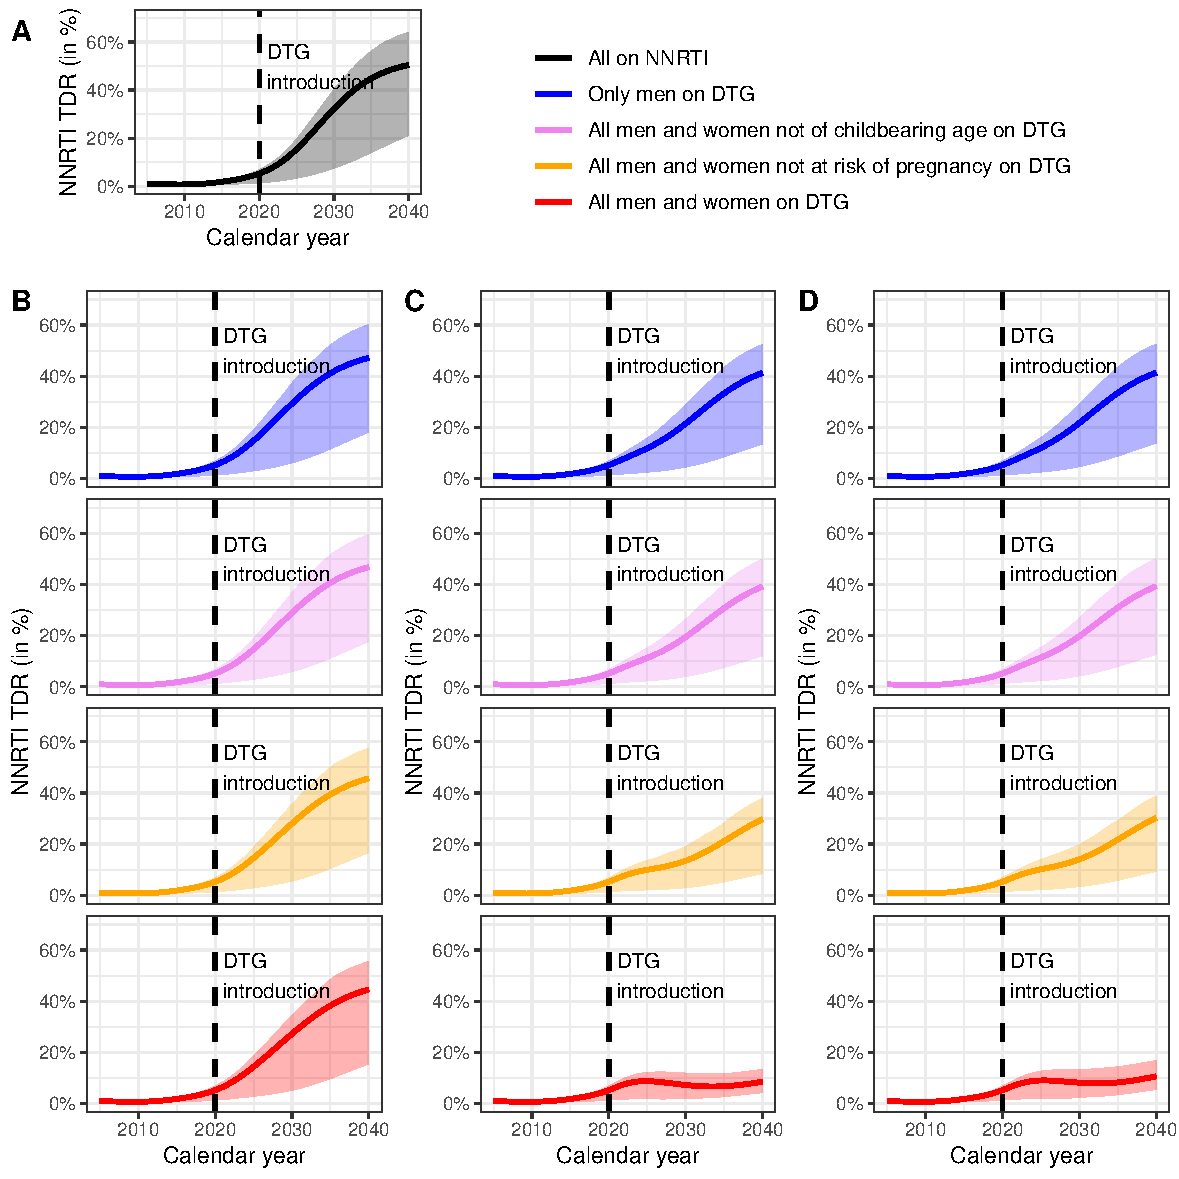
\includegraphics[width=16cm]{../figures/sens_uncertainty.pdf}
   \caption{Level of NNRTI PDR according to different levels of DTG-eligible women (colors), and different strategies of DTG-introduction. Panel A: no DTG-introduction; panel B: DTG used as a first-line regimen; panel C: DTG used for all patients; panel D: DTG used for all patients, assuming an OR of failure of 2 when having NRTI-resistance. The solid lines correspond to the simulations with the fixed parameter values and the shaded areas represent the 95\% sensitivity ranges.}\label{fig:sensitivity_range}
\end{figure}

\begin{figure}[h!]
\centering
   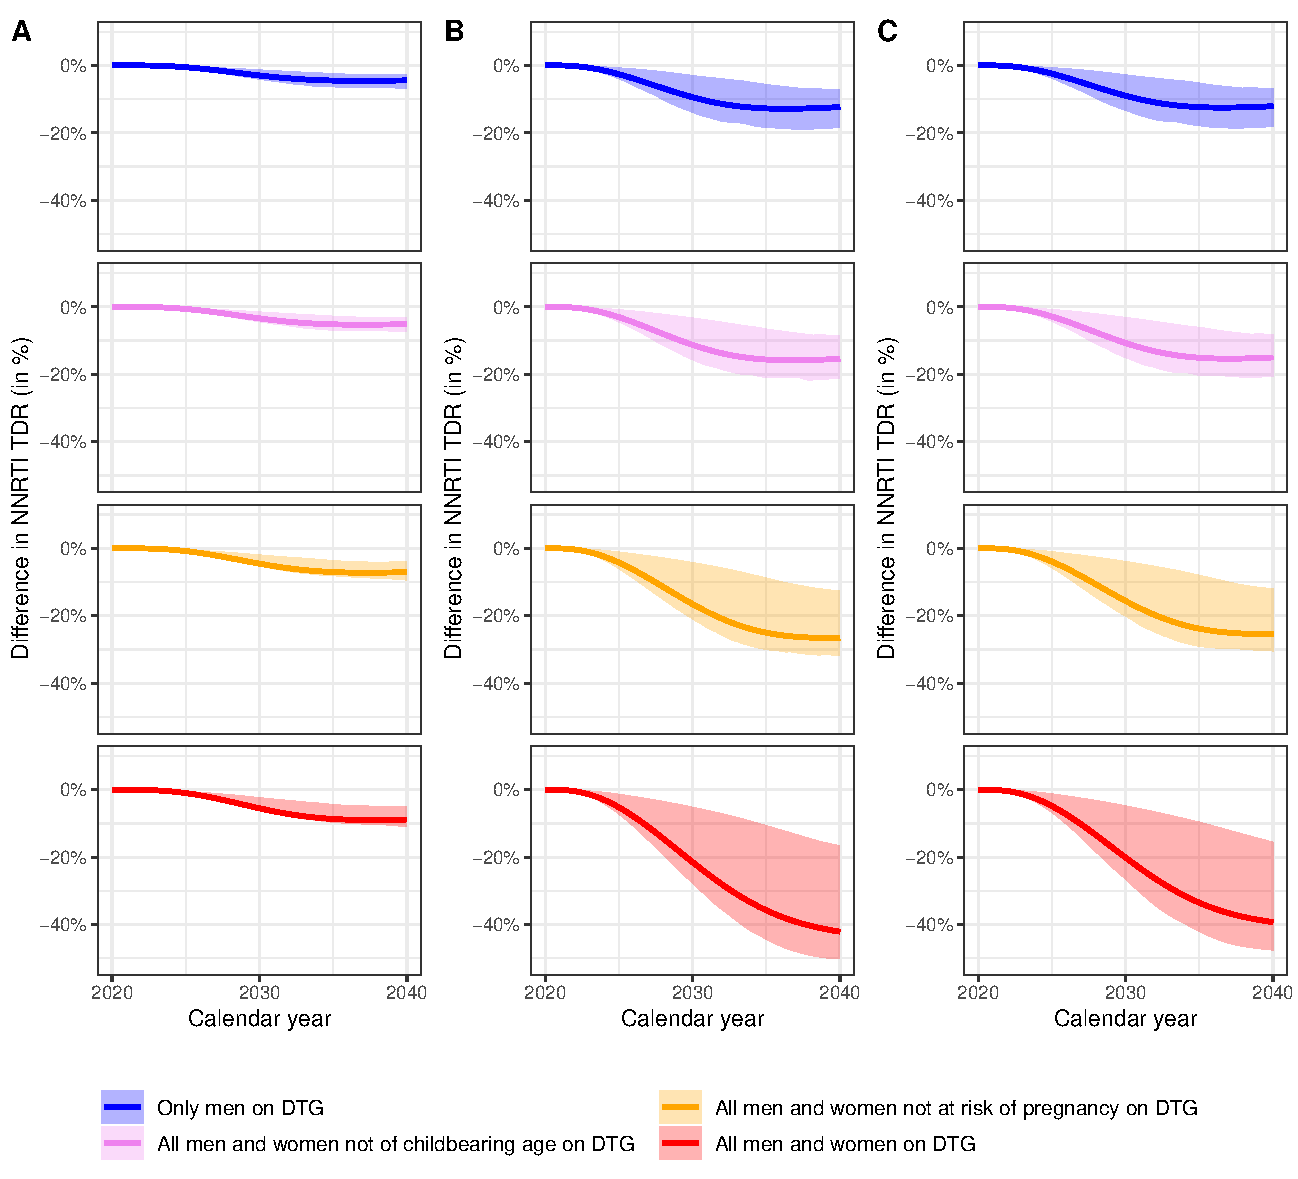
\includegraphics[width=16cm]{../figures/sens_diff_uncertainty.pdf}
   \caption{Difference in level of NNRTI PDR from 2020 to 2040 between the different strategies of DTG-introduction and the scenario where DTG is not introduced. Panel A: DTG used as a first-line regimen; panel B: DTG used for all patients; panel C: DTG used for all patients, assuming an OR of DTG-failure of 2 when having NRTI-resistance. The solid lines correspond to the simulations with the fixed parameter values and the shaded areas represent the 95\% sensitivity ranges.}\label{fig:diff_sensitivity_range}
\end{figure}

\subsection{Effect of no Treat-All policy}
We previously assumed that the Treat-All policy increased the treatment initiation rates for people with $CD4>200\text{ cells}/\mu L$ from 2017 to 2022. Here, we investigated the scenario where the Treat-All policy does not have any impact on the treatment initiation rates (which is equivalent to assuming no Treat-All policy, see Fig\ref{fig1_notreatall}). Globally, assuming a Treat-All policy increases the levels of NNRTI PDR for each scenario, but does not change our conclusion (see Fig\ref{fig2_notreatall}).

\begin{figure}[h!]
\centering
   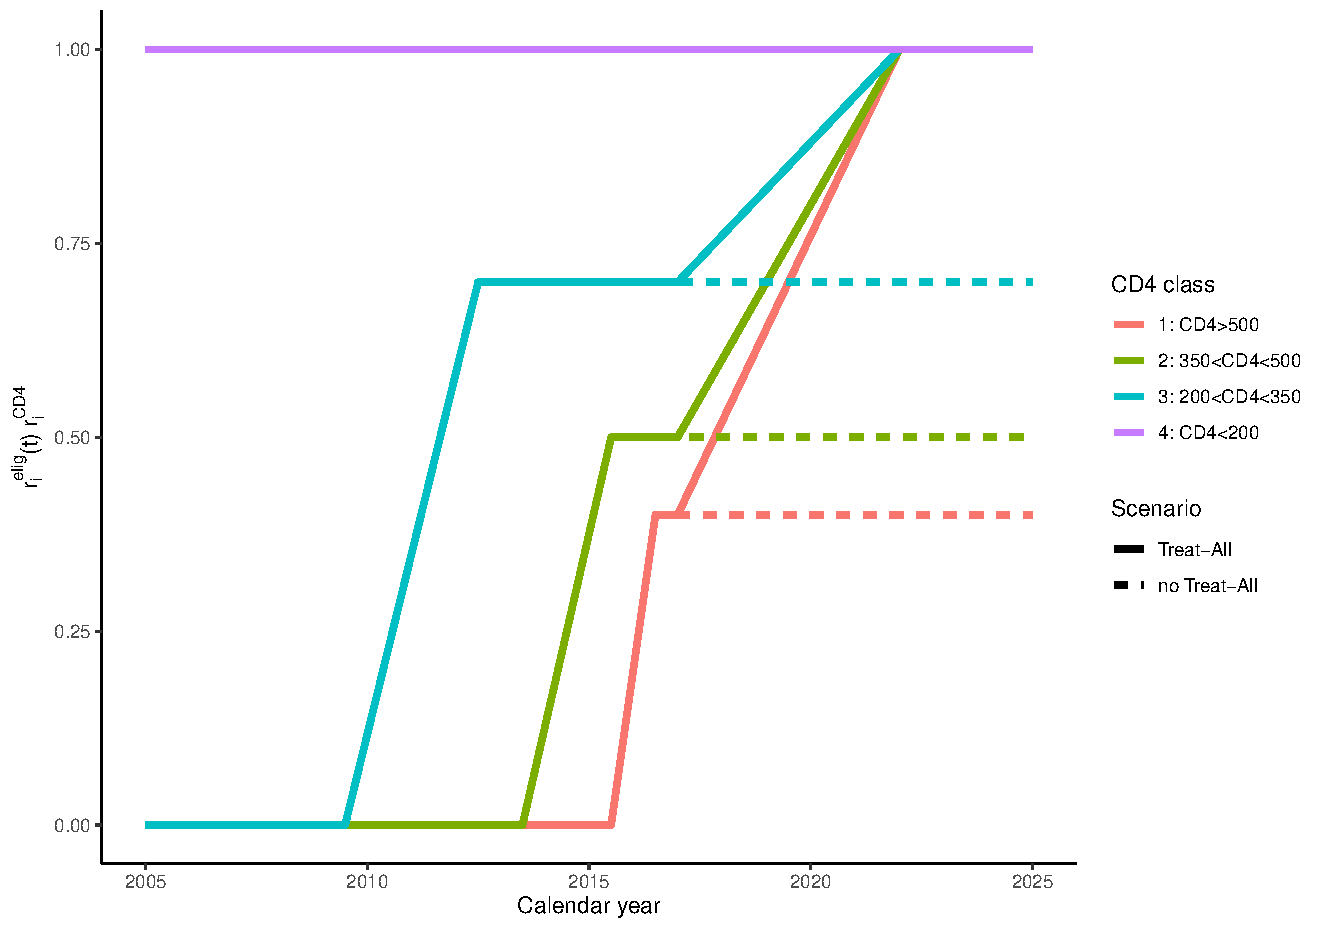
\includegraphics[width=14cm]{../figures/dtg_plot_treatrate2.pdf}
   \caption{$r^{elig}_i(t) \cdot r^{CD4}_i$ represents the level of treatment eligibility $r^{elig}_i(t)$ multiplied by $r^{CD4}_i$, representing the decrease in treatment initiation rate in CD4 class $i$ relative to the fourth CD4 class ($CD4<200 \text{ cells}/\mu L$). In the scenario where we assumed no impact of the Treat-All policy on the treatment initiation rates, the rates remain unchanged from 2016.}\label{fig1_notreatall}
\end{figure}

\begin{figure}[h!]
\centering
   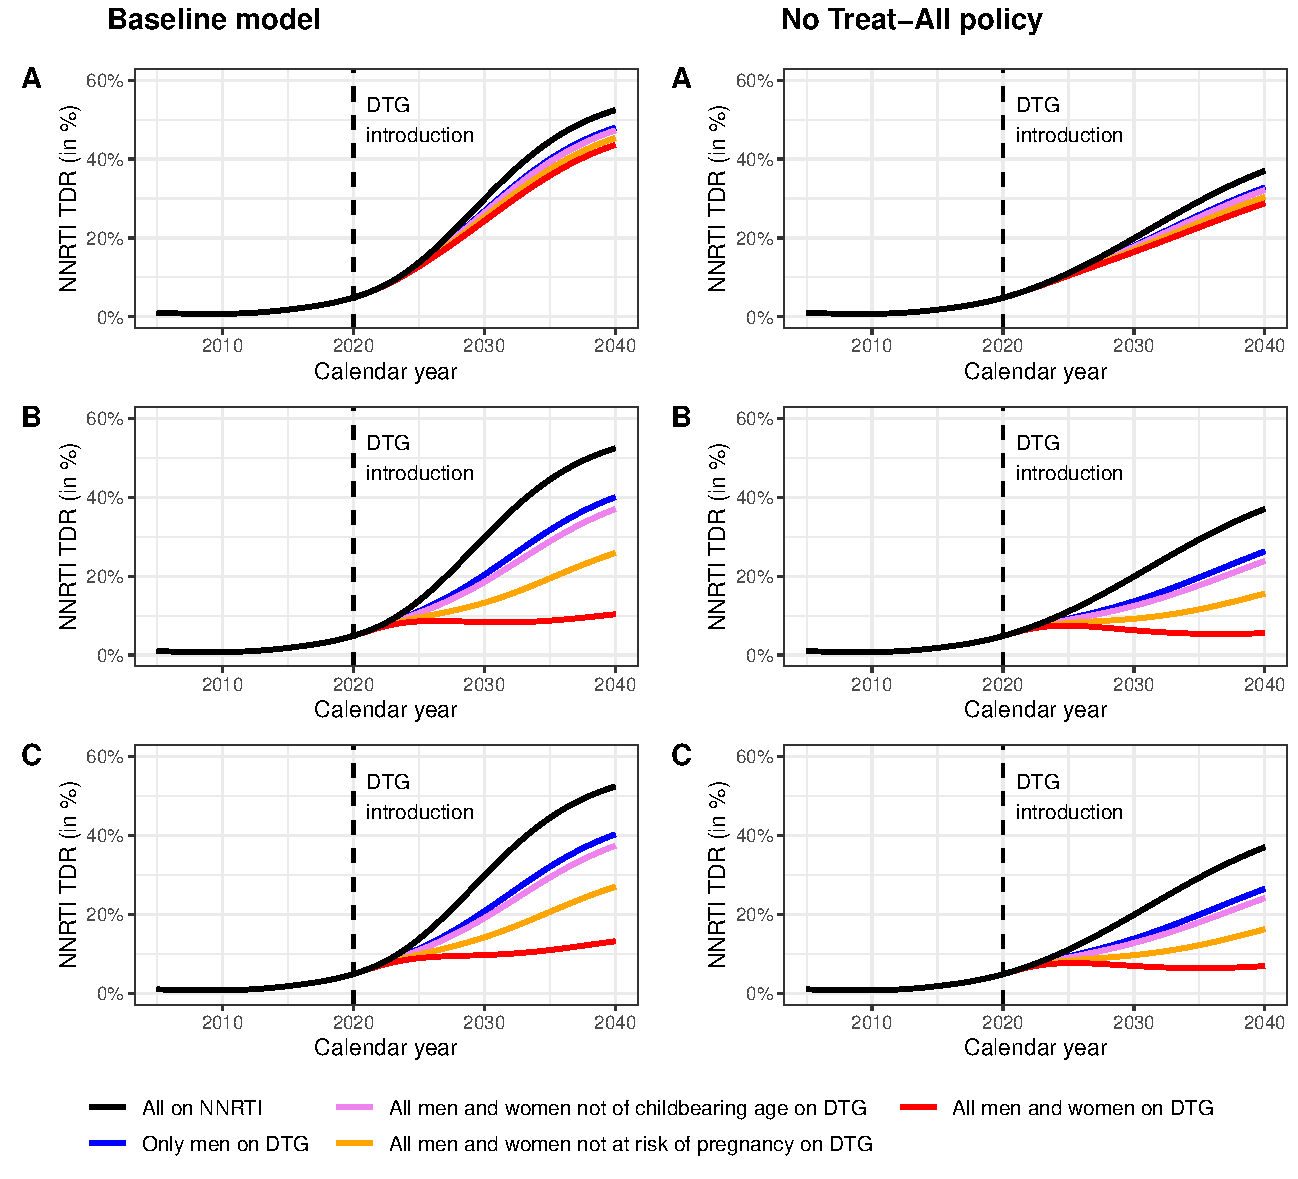
\includegraphics[width=16cm]{../figures/sens_notreatall.pdf}
   \caption{Levels of NNRTI resistance when assuming increase in treatment initiation rates due to the Treat-All policy ("Baseline Model") and when assuming identical treatment initiation rates from 2017 ("No Treat-All policy"). Dolutegravir is introduced in 2020 under three scenarios: DTG as first-line regimen for ART-initiators (panel A), DTG for all patients (panel B), DTG for all patients, assuming an OR of failure of 2 when having NRTI-resistance (panel C), and with different eligibility criteria for women (colors).}\label{fig2_notreatall}
\end{figure}
\newpage
\subsection{Effect of treatment interruption}
We introduced treatment interruption rates for the three ART regimens. Table \ref{tab_int} shows these rates estimated from IeDEA-SA data \cite{Egger2012}. The introduction of treatment interruption did not substantially change the results (see Fig \ref{fig_int}).

\begin{table}[H]
\centerline{
	\begin{tabular}{llllll}
		\hline\\[-0.4cm]
		Parameter & Description & \multicolumn{4}{c}{CD4 class}\\ 
		& & $1$ & $2$ & $3$ & $4$\\[0.1cm]
		\hline\\
		$1/\gamma_{T\rightarrow D}$ & Time from $T_1/T_2/T_3$ to $D$ & 414 & 322 & 172 & 156\\
		$1/\gamma_{S\rightarrow D}$ & Time from $S_1/S_2/S_3$ to $D$ & 2069 & 1241 & 759 & 368\\
		$1/\gamma_{F\rightarrow D}$ & Time from $F_1/F_2/F_3$ to $D$ & 621 & 478 & 285 & 129\\[0.1cm]
		\hline
	\end{tabular}
}
\caption{Treatment interruption rates. Rates are in $\text{month}^{-1}$}
\label{tab_int}
\end{table}

\begin{figure}[h!]
\centering
   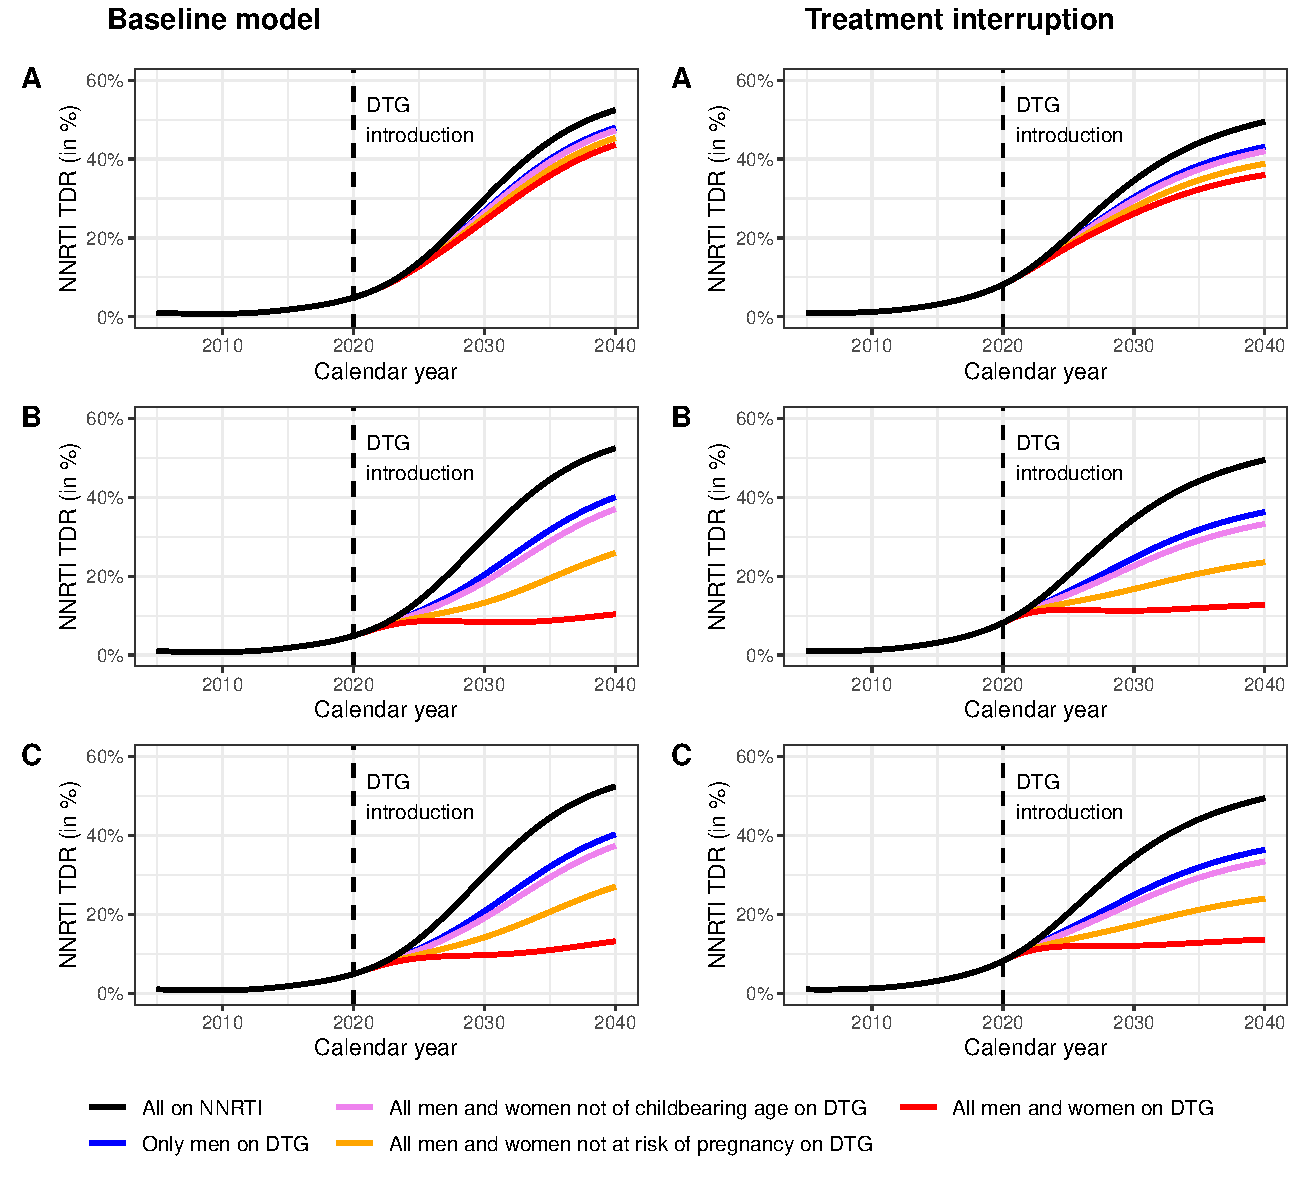
\includegraphics[width=16cm]{../figures/sens_treatinterruption.pdf}
   \caption{Levels of NNRTI resistance using the baseline model ("Baseline Model") and when including treatment interruption ("Treatment interruption"). Dolutegravir is introduced in 2020 under three scenarios: DTG as first-line regimen for ART-initiators (panel A) or DTG for all patients (panel B), DTG for all patients, assuming an OR of failure of 2 when having NRTI-resistance (panel C), and with different eligibility criteria for women (colors).}\label{fig_int}
\end{figure}
\newpage
\subsection{Effect of NRTI-resistance and higher efficacy of DTG}\label{sec_analysis}
We assessed the impact of NRTI resistance and higher efficacy of DTG-based regimen on the level of NNRTI PDR. We investigated three different scenarios regarding the impact of NRTI-resistance: 1) no impact (i.e OR of failure between NRTI-susceptible and -resistant individuals equals 1), 2) OR=2, and 3) OR=5. A meta-analysis comparing DTG-monotherapy with DTG-dual therapy found an odds ratio of failure of 13.9 after 48 weeks (8.9\% vs 0.7\% of failure, respectively). However, we expect lower difference between NRTI-resistant and -susceptible individuals, as some activity of the NRTI-backbones are observered even in resistant individuals \cite{Hakim2018}. Another study comparing DTG-efficacy according to the presence of specific NRTI-mutations found a HR of 3.23 (95\%CI: 0.27-38.40) when having the K65R mutation and a HR of 0.99 (95\%CI: 0.19-5.21) when having the M184V, suggesting low impact of NRTI-resistance on DTG-failure.

We also investigated three different scenarios regarding the efficacy of DTG compared with NNRTI: 1) OR of failure between NNRTI- and DTG-based regimen of 1.02, 2) OR=2, and 3) OR=5. The first scenario refers to the results of the NAMSAL study after the adjusting for CD4 counts (see Section \ref{sec:nrti_res}). The two other scenarios were investigated in view of the higher efficacy of DTG compared with NNRTI found in some studies \cite{Snedecor2019}.


\begin{figure}[h!]
\centering
   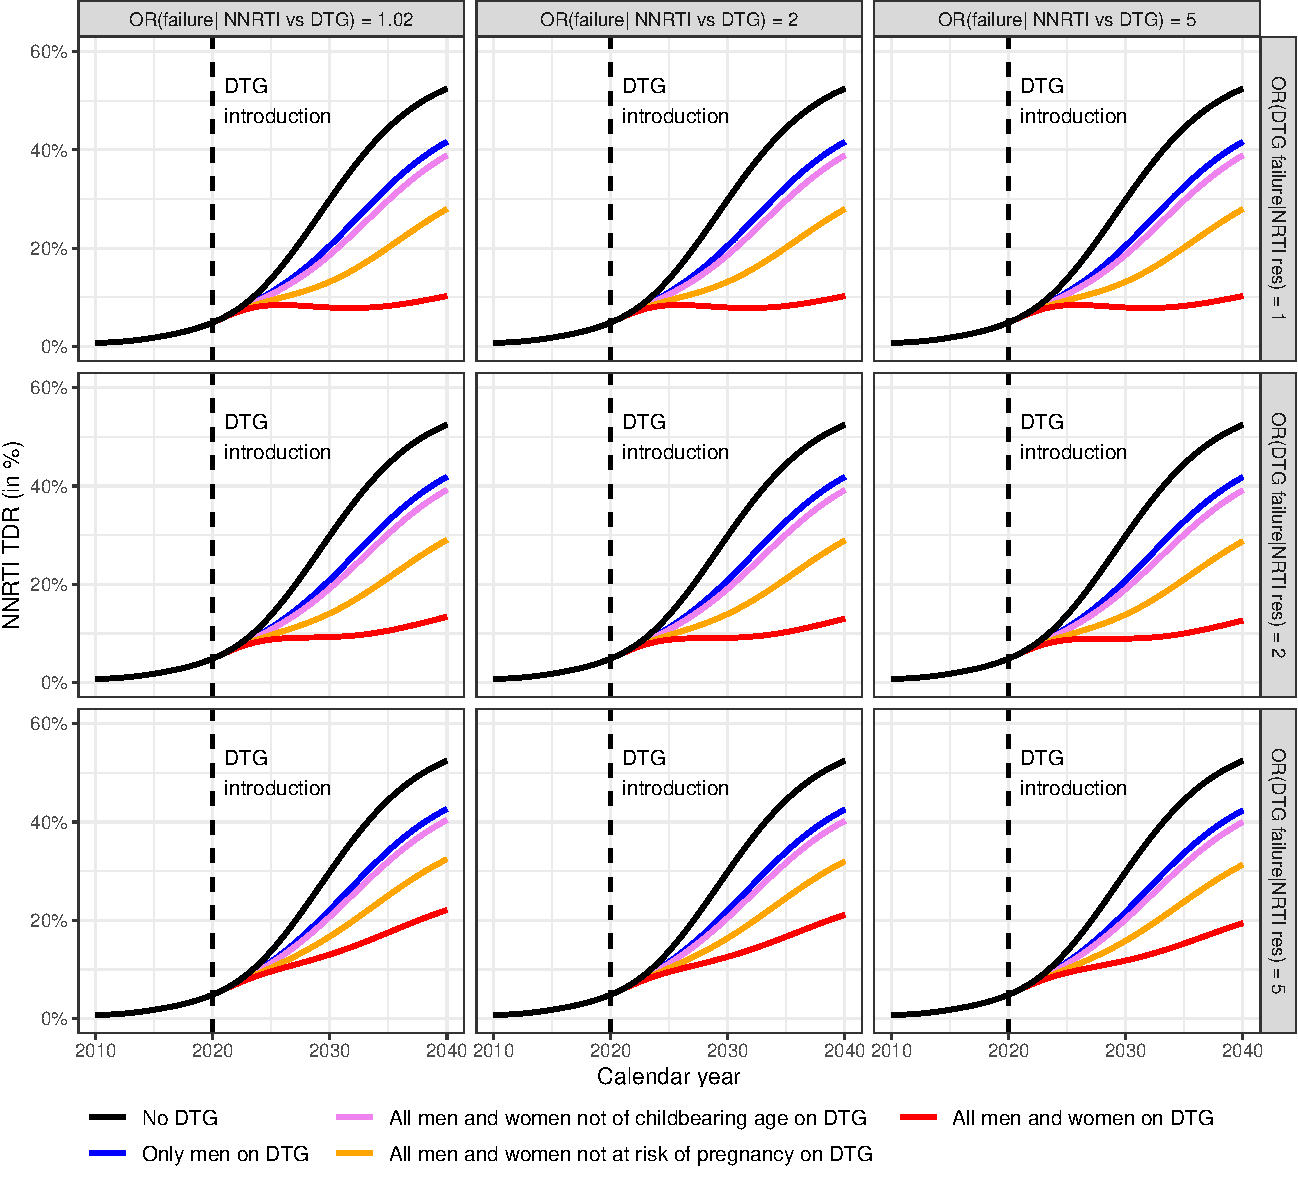
\includegraphics[width=16cm]{../figures/sens_nrti_res.pdf}
   \caption{Levels of NNRTI TDR from 2010 to 2040, when assuming that DTG is used both as  first-line and switch regimens. Different impacts of NRTI-resistance on DTG-failure (horizontally) and different DTG-efficacies (vertically) are investigated.}\label{figure2}
\end{figure}

\newpage
$ $
\newpage
\bibliography{C:/Users/ahauser/Documents/Step2/Step2_revised/manuscript/dtg_bib_supmat}
\end{document}